% Please do not change the document class
\documentclass{scrartcl}

% Please do not change these packages
\usepackage[hidelinks]{hyperref}
\usepackage[none]{hyphenat}
\usepackage{setspace}
\usepackage{graphicx}
\doublespace

% You may add additional packages here
\usepackage{amsmath}

% Please include a clear, concise, and descriptive title
\title{The history of digital facial replication including methods used and problems that arose}

% Please do not change the subtitle
\subtitle{Comp130 - Research project}

% Please put your student number in the author field
\author{1506919}

\begin{document}

\maketitle

\abstract{This paper will look into the history of facial replication, focusing especially on the methods used including the problems occurred. The introduction explains why it is important for digital faces to be realistic, then the paper will look at the articles from the past 40 years drawing a comparison of results and looking into how the methods changed from paper to paper over the years, each hoping to make it better, using images to help explain the most important part of the methods which can be lengthy and confusing.}

\section{Introduction}

Photorealism is a very important factor to take into account for creating characters for digital games, if the game has an emotional plot line the more realistic the facial expressions of the characters whether happy or sad, the more likely the player will become emotionally invested in the story, the game will feel more immersive\cite{Guardian2015}\cite{schneider2007exploring}. Rockstar Games LA Noire\cite{games2011noire} is a good example of using expressions within a digital game as the story involved judging an NPCs expression to decide if what they have said is true or false, is the character angry, happy or upset?\cite{liu2013game}

In this paper I will look into the history of digital face replication to find how the methods evolved, the problems the creators experienced. The conclusion will summarise what was learnt in those years, the importance of what the authors did and looking at their papers what we can expect in the future.

\section{History}

Frederick Ira and Parke wrote a paper in 1976 called A parametric model for human faces, this is one of the first papers written about trying to recreate a three dimensional actors face digitally and animate to show a range of emotions. The main motivation for this project was that it was challenging they noticed how the face is an important subject for art and photographs they hoped computer graphics would have a place in that field. Before this paper two dimensional faces had been created and manipulated to show expressions but three dimensional faces created out of polygonal surfaces had been very difficult to animate because a collection of three dimensional data containing every single expression was needed\cite{parke1974parametric}.

Stephen M. Platt and Norman I. Badler worked on creating a digital representation of a human to preform American sign language actions, creating a digital body using a rigid model presented no problems but the the face is not rigid and therefore cannot use the same model, instead they used the facial action recognition to simulation system\cite{platt1981animating}.

Lance Williams intended to add to and improve facial mapping, texture and expression in his paper using the current technologies available at the time, Performance-Driven Facial Animation was written (1990), taking into account the methods described in papers written by Frederick Ira, Parke\cite{parke1974parametric}, Stephen M. Platt and Norman I. Badler\cite{platt1981animating}, Brennan, Susan Elise\cite{brennan1982caricature}, Burrson, Nancy, and Schneider, Thomas\cite{burson1981method}, and the methods they used for replicating faces digitally to create a electronic mask technology that would make replicating faces digitally easier than before\cite{williams1990performance}.

\section{Methods and problems for facial replication}

Frederick Ira, Parke created a method for replicating faces with polygons called the parmetric controlled model (Figure 1), by using a model of a head that was then created digitally as a guide the peramteres can be changed to replicate an actor, the peramters would have been manually put into the model.

\begin{figure}[h]
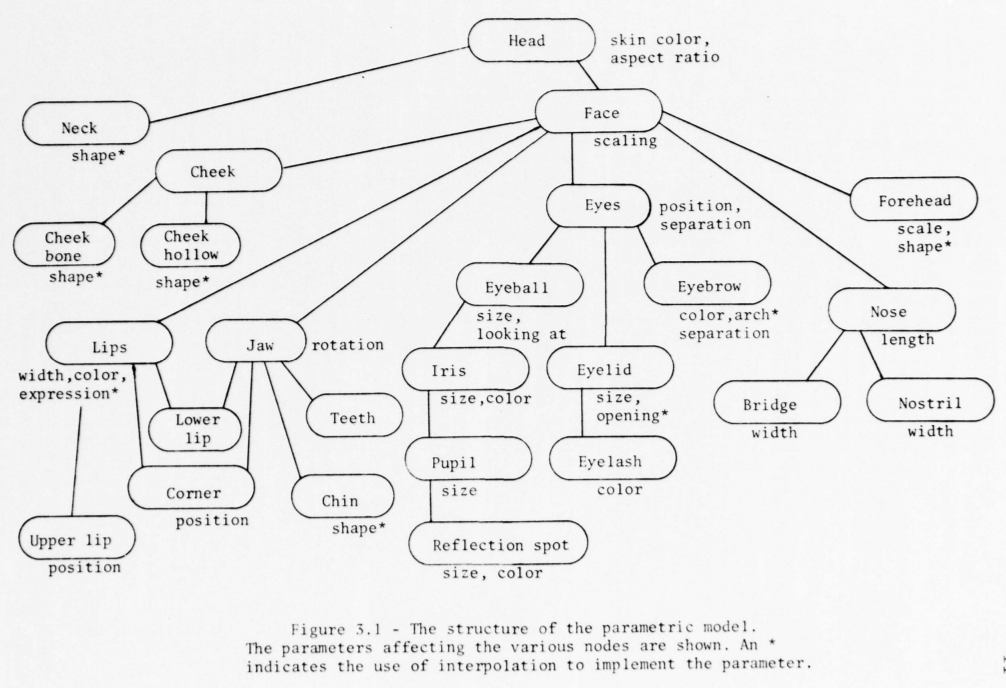
\includegraphics[width=12cm]{Parametric.png}
\caption{The parametric model \cite{parke1974parametric}}
\label{fig:Model1}
\end{figure}

Animating the face to show emotions meant having to individually code the changing parameters over a set time for example to create a smile would mean changing the height of the corners of the mouth gradually over the space of one second. To replicate speech an actor was filmed reading a speech and their voice recorded desperately, the mouth movements were replicated by taking note of the parameter changes and coding these changes with delays where needed to get the animation as close as possible. The drawbacks of this method is that the animation quickly became over animated and played much slower, looking unnatural also the whole process of having to change each parameter for every letter is extremely time consuming. Although parametric model was not an ideal method to replicate faces, it provided a good start to build on for the future\cite{parke1974parametric}.

The facial action recognition to simulation system (Figure 2) used by Stephen M. Plait and Norman I. Eadler used an input from a camera controlled by the computer to record an actors facial movement, focusing on muscles within the face, this information goes to the camera processor which turns the facial muscle movement into a notation representation, paying attention to facial movement that effect other features such as the cheeks changing shapes when the lips move to create words. The notation is given to the internal model manipulator which turns the information into structures used by the simulator, the simulator runs is responsible for tensing and relaxing muscles from frame to frame depending on what the previous movement was, this is important as the face is saved in its current state between the frames, it can also runs two movements parallel to one another if necessary to produce the final output\cite{platt1981animating}.

\begin{figure}[h]
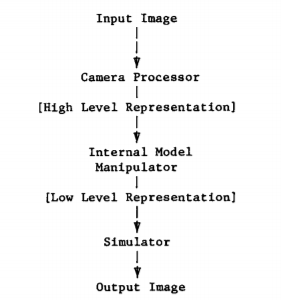
\includegraphics[width=8cm]{Facial_action_recognition_to_simulation_system.png}
\caption{Facial action recognition to simulation system \cite{platt1981animating}}
\label{fig:Model2}
\end{figure}

Comparing the parametric model to the facial action recognition to simulation system, the latter was created 7 years after Frederick Ira and Parke first published their paper and most of the problems he came across have been solved, slow playback due to over animation has been solved and having to change each parameter manually has been replaced by the by the camera processor. Although the problems from the parameter model has been solved Stephen M. Plait and Norman I. Eadlers facial action recognition to simulation system has its own range of problems, the way the face is created at in the system uses muscle with no solid bone sheet underneath so when the face preforms some sudden change of movement it appears that the muscles are going through where the bone structure would be leading the face to become distorted for a certain amount of frames. Jaw movement like speaking, along with cheeks being puffed in or out is not an ability the facial action recognition to simulation system is capable of and cartilaginous areas are prone to slight movement when the muscles around that area are tightened which results in unrealistic movement. All of the problems presented were handled better with the previous parametric model.

Lance Williams uses the latest technology available at the time (1990) to improve digital facial replication. Using the help of the company Cyberware Inc they gathered digital data from a plaster cast of a dancers head and sent back a tape which held the data for the head including the features positions and sizes. Face Software Inc was tasked with taking a composite photograph of the whole head and using the data from the plaster cast Face Software Inc was able to manipulate the dancers face to match the position of the features from the scanned head, making the facial replication simpler. The next steps included a lot of filtering to make the photographs look realistic when they are added to the digital head model which included smoothing textures and reducing noise, though these processes would ideally be automatic including the work done by Face Software Inc in the end technology, Lance Williams created an alternative way to do all the texturing at once by using a peripheral camera to take a photo of the whole head then software was created to add texture, polygon engines where then used for mesh tessellation. Finally the head had to be animated, the digital face expressions were controlled using a live actor and video-based tracking, retroreflective material applied to the actors face (Figure 3) and corresponding crosses where placed on the digital head (Figure 4).

\begin{figure}[h]
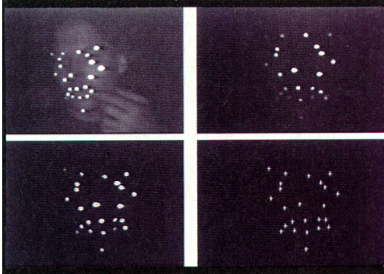
\includegraphics[width=5cm]{Live_actor_with_tracking_retroreflective_material.png}
\caption{Live actor with tracking retroreflective material \cite{williams1990performance}}
\label{fig:Model3}
\end{figure}

\begin{figure}[h]
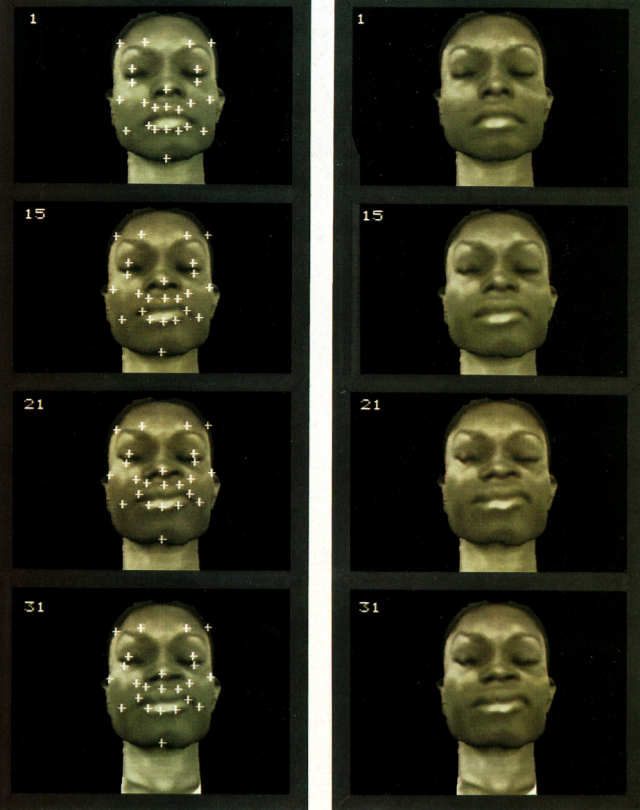
\includegraphics[width=8cm]{Movement_from_Actor_applied_to_digital_Face.png}
\caption{Movement from the actor applied to the digital face \cite{williams1990performance}}
\label{fig:Model4}
\end{figure}

Lance Williams concluded that using a live actor with video-based tracking was definitely the future for animating digital faces and suggests further research should be done on how well this would work with a face that is completely different from that of the actor, comparing this to the work of Frederick Ira, Parke and Stephen M. Platt, Norman I. Badler both of who had problems with the face becoming distorted and large amounts of time spent manually changing the face parameters to exhibit expressions, video-based tracking seems to have eradicated both of these problems. Of course this system was not able to open the digital heads mouth to replicate the movements of speech or eyelid movement, which was also a problem for the facial action recognition to simulation system but not by the parametric model because the data for this model was entered manually more attention was paid to try and make the model move as lifelike as possible, whereas Stephen M. Platt, Norman I. Badler seemed to pay more attention to replicating expressions, Lance Williams did not include mouth or eye movement in his paper though in the conclusion does mention that tests were carried out and found the eyelids to be easily trackable using the video-based tracking system.

\section{Conclusion}

The papers discussed here are important in the evolution of replicating faces within a digital environment, as only once people have explored certain methods, whether they resulted in success or fail, can a method be developed and perfected for use in the future. As their papers show, there seemed to be a positive correlation between the development of technology and the realism of replicated faces becoming easier to create. The development of technology never stops, so in the future the methods for creating digital faces will continue to get easier and more detailed every year.

\bibliographystyle{ieeetran}
\bibliography{references}

\end{document}
